\documentclass[conference]{IEEEtran}
\IEEEoverridecommandlockouts
% The preceding line is only needed to identify funding in the first footnote. If that is unneeded, please comment it out.
\usepackage{cite}
\usepackage{amsmath,amssymb,amsfonts}
\usepackage{algorithmic}
\usepackage{graphicx}
\usepackage{textcomp}
\usepackage{xcolor}
\usepackage{subfigure}
\def\BibTeX{{\rm B\kern-.05em{\sc i\kern-.025em b}\kern-.08em
    T\kern-.1667em\lower.7ex\hbox{E}\kern-.125emX}}
\begin{document}

\title {Recipient Detection in Historical Documents}

\author{\IEEEauthorblockN{Alex Felker}
\IEEEauthorblockA{\textit{Friedrich-Alexander-Universität Erlangen-Nürnberg} \\
Erlangen, Germany\\
alex.felker@fau.de}
}

\maketitle

\begin{abstract}
Both handwritten text analysis and image segmentation are widley used approaches in the machine learning community, which have already delivered good results on certain tasks. The goal of this work is to combine both approaches to generate additional benefit without changing the underlying data. The task to be solved is the recognition of recipient regions in the letters from the Nuremberg letterbooks from the 15th century. To achieve this goal, the semantic features in the text itself as well as the visual features of the letter pages should be analysed and combined. To extract the semantic features, this work utilizes a deep learning based image to text model, followed by an also deep learning based text classifier. The output of this text classifier is then used to construct a mask with recipient predictions. In order to extract the visual features, a U-Net architecture is used to solve the segmentation task. Both resulting masks were then combined, and the results were subsequently evaluated. The results obtained show that a minimal performance boost was achieved compared to the segmentation using the standalone U-Net. However, this performance boost is not completely satisfactory, which is why we have to work on the quality of the text classification or the combination method in the future.
\end{abstract}

\section{Introduction}
In our modern society, almost all written texts are digitalized and thus easy for machines to interpret. Extracting information from older means of communication, such as letters, requires significantly more effort. This problem constitutes the larger scope of this work. More specifically, the Nuremberg letters of correspondences from the 15th century will be examined in more detail to make it easier for historians to tag the recipients of individual letters. For this purpose, deep learning techniques are utilized to automatically recognize the lines of a letter with recipient information. The main goal of this work is to combine both visual and semantic features of a letter to obtain the recipient. \newline
To achieve this, section \ref{data} covers the data analysis and the necessary preparation steps to make the data usable for both visual and semantic feature processing. In order to determine the semantic features, the handwritten lines must be converted to machine-interpretable text. This will be done by a deep learning-based neural network architecture, which will be explained in section \ref{sem_feat}. After this, the text will be classified to recipients- and non-recipients, using a deep learning classifier, which will also be explained in more detail in section \ref{sem_feat}. This classifier is then used to create a mask for the whole page based on the classification probabilities. On the other hand, section \ref{visual_feat} describes the extraction of the visual features which will be done by a U-Net \cite{ronneberger2015unet}. The feature mask obtained in this way is then combined with the mask created by the recipient classification, which is described in more depth in section \ref{combinded_feat}. After a short overview of training settings and hyperparameters in secion \ref{training}, this work continues with the evaluation in section \ref{evaluation}. The main aspect here will be the comparison of the line detection performance of the standalone U-Net and the combined prediction mask. The paper then finishes with a discussion of the results in section \ref{discussion} and a brief conclusion with an outlook in section \ref{conclusion}.

\section{Dataset analysis and preprocessing}\label{data}
This section gives a brief overview of the data used and how they were made available for the various models.

\subsection{Dataset analysis}

\begin{figure}[htbp]
    \centering
    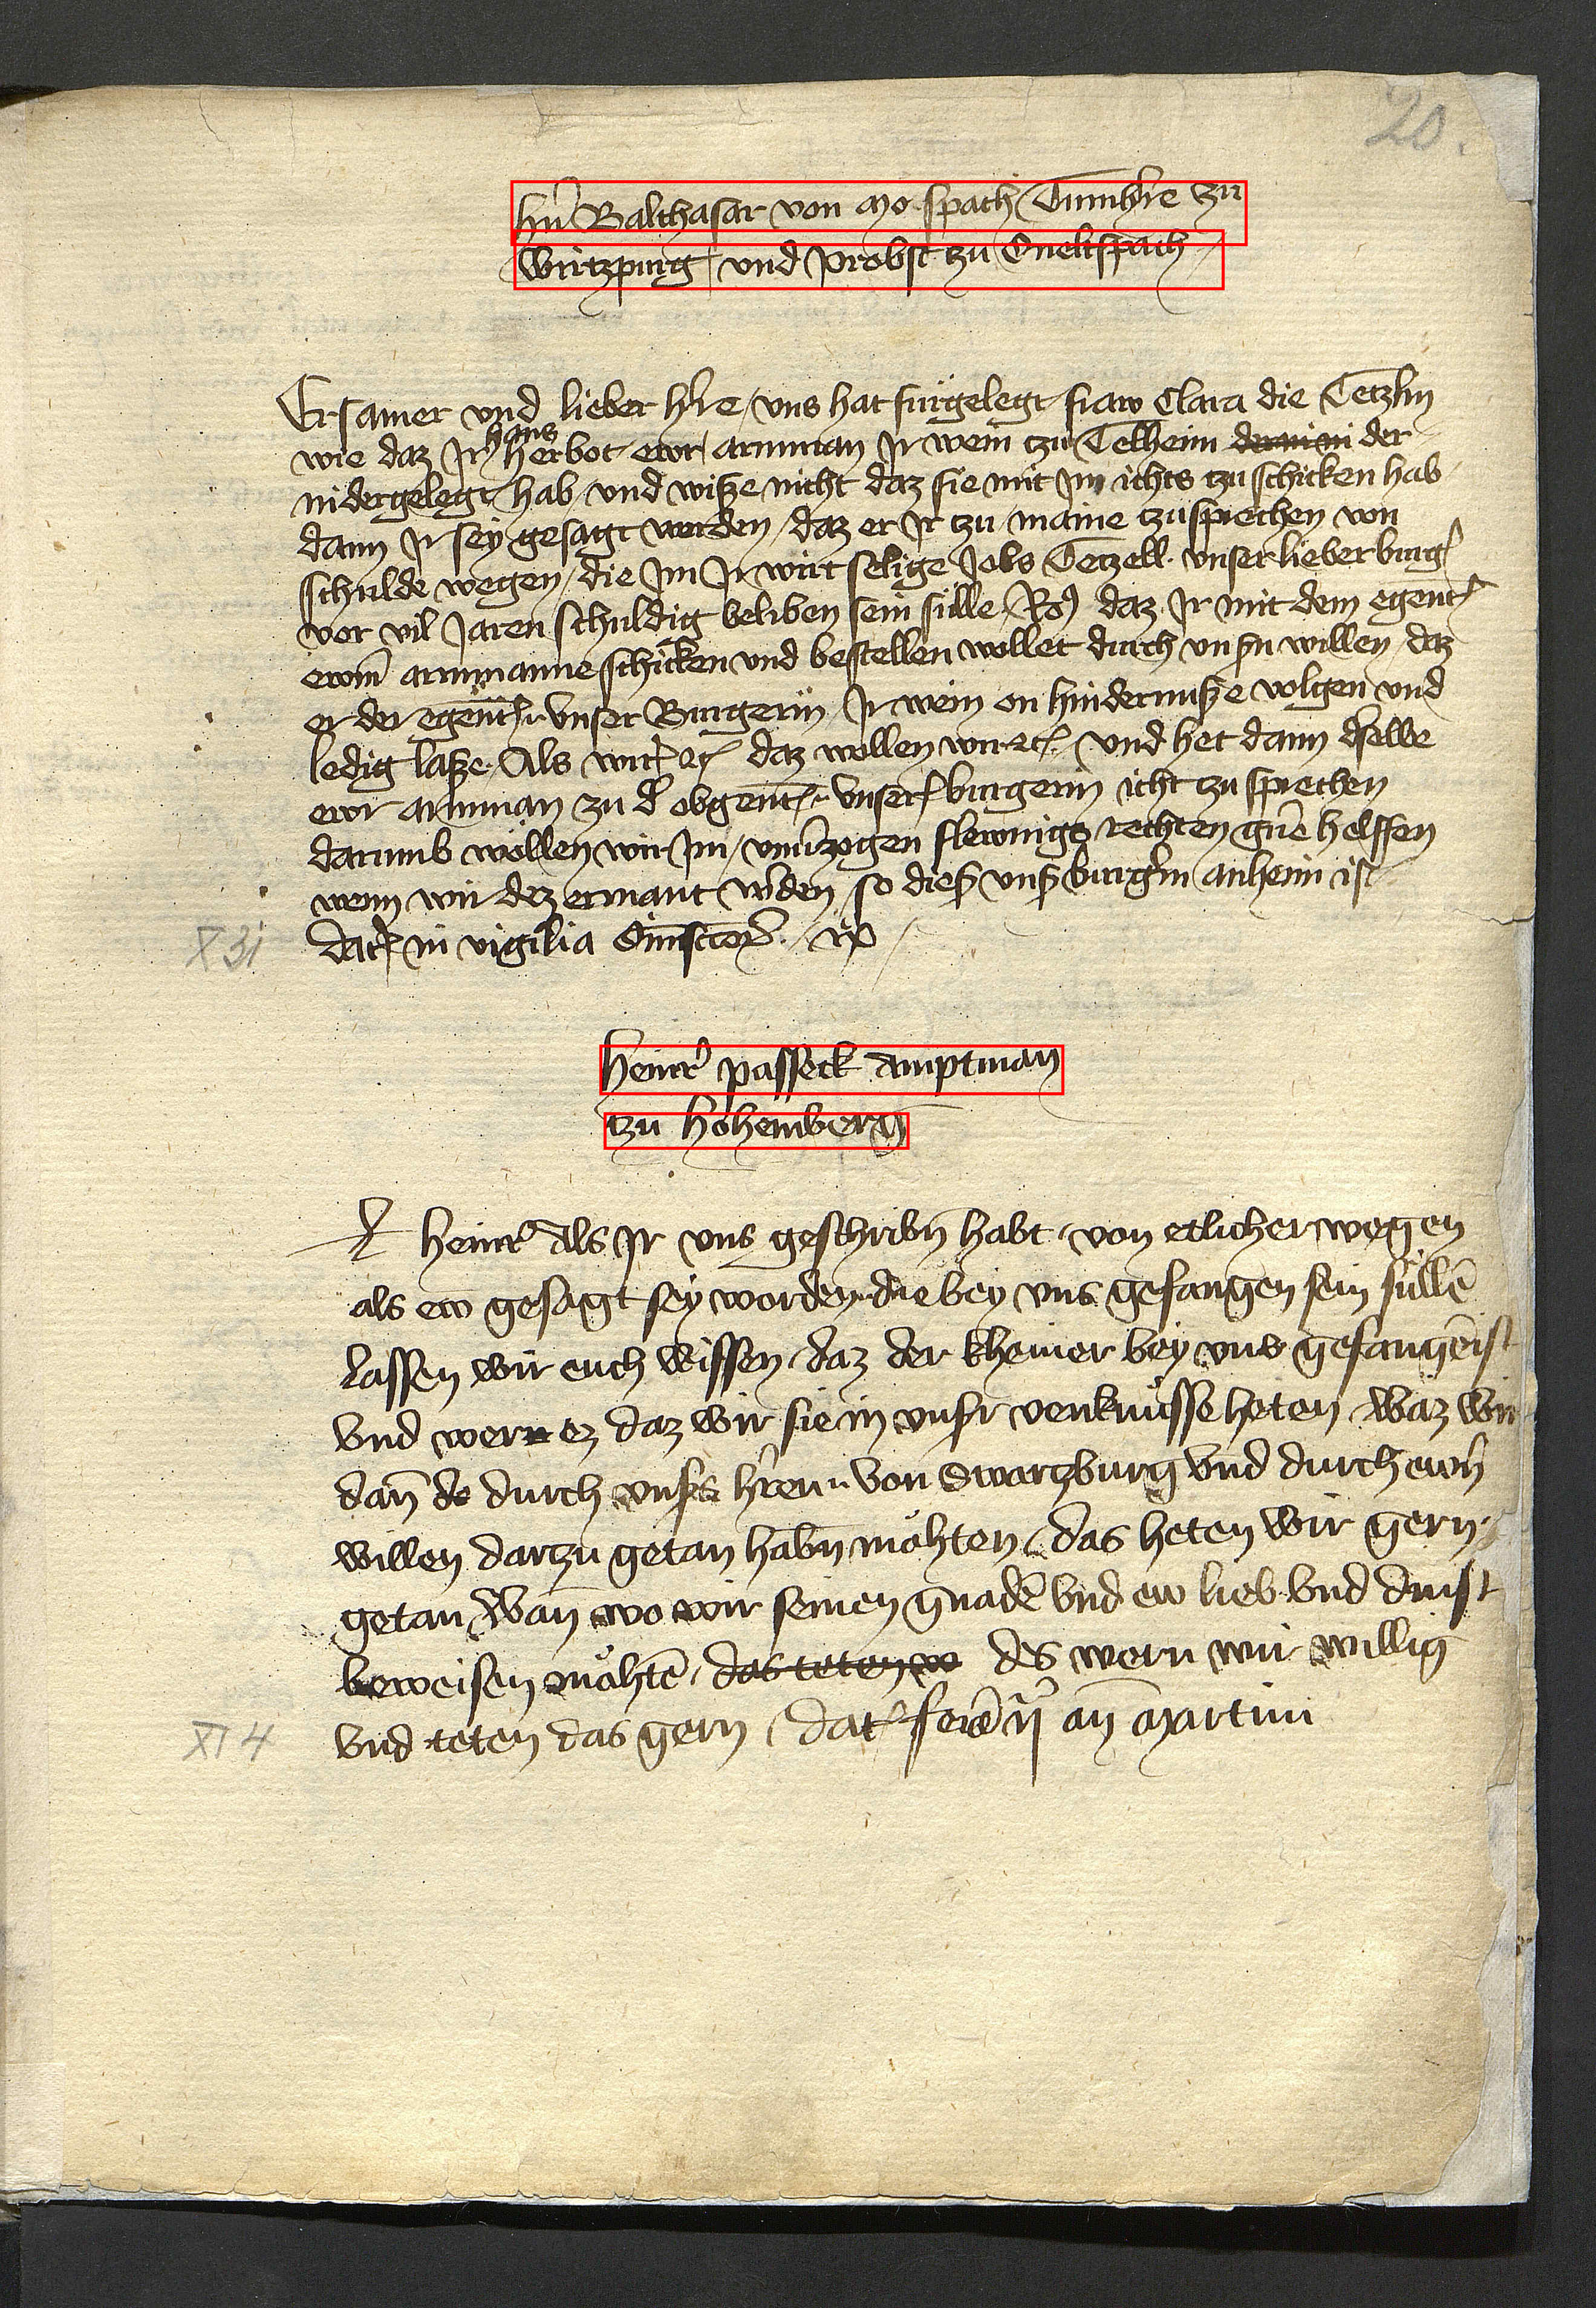
\includegraphics[width=0.5\textwidth]{figures/example_page.png}
    \caption{Example data excerpt with recipient highlightning}
    \label{example}
\end{figure}

The train, validation and test dataset consists of 1.548 pages from four different volumes of the Nuremberg letterbooks from the 15th century. An example page can be seen in Fig. \ref{example}, where the red boxes are indicating the recipient lines. Each page contains on average about 30 lines, including information such as the contained text and the recipient label. In addition, the exact position and size are annotated for each line. These information are provided by induvidual XML files for each page. The data to be used for the actual use case, however, has no information about the textual content or recipient label.
The alphabet used for the semantic feature extraktion is constructed by all letters that occur in the dataset with additional padding and blank token to be able to utilize the ctc loss, which will be further explained in section \ref{sem_feat}.

\subsection{Dataset preprocessing}

\begin{table}[htbp]
\caption{Overview random data augmentation for semantic features}
\begin{center}
\begin{tabular}{|c|c|}
\hline
\textbf{\textit{Method}} & \textbf{\textit{Probability}}  \\
\hline
Elastic distortion \cite{yousef2020origaminet} & 0.6 \\
\hline
Random transformes \cite{yousef2020origaminet} & 0.6 \\
\hline
Dilation \& Erosion & 0.6 \\
\hline
Contrast adjustment & 0.6 \\
\hline
Random perspective \cite{NEURIPS2019_9015} & 0.6 \\
\hline
\end{tabular}
\label{data_aug}
\end{center}
\end{table}


In order to make the dataset work for both, the semantic and the visual feature extraction, two different data preprocessings are required. For the semantic features, the individual lines must be cut out of the pages, using the position and size annotations provided by the corresponding XML tag. The cut-out lines are then augmented, binarized and resized to a fixed height of 64 pixels. Binarization was applied by utilizing sauvola thresholding proposed in \cite{SAUVOLA2000225}. The mentioned random augmentation methods can be obtained from table \ref{data_aug}. Moreover, a zero padding, matching the widest line for each batch, is applied to make the data usable for the model architecture. The augmented and padded lines are then provided with the ground true text and recipient label information. An example of a fully processed line image can be seen in Fig. \ref{line_img}. \newline

\begin{figure}[htbp]
    \centering
    \includegraphics[width=0.5\textwidth]{figures/line_img.png}
    \caption{Fully processed line image}
    \label{line_img}
\end{figure}

With the U-Net, a separation of the lines is not required, which is why a different data preprocessing had to be implemented here. The architecture takes whole letter book pages as input, which are simply resized to a fixed width and height of 256 pixels. As a target, a recipient matrix was created for each page, which has ones in areas with recipients and zeros otherwise. These matrices were then resized to the same height and width as the input. Additional data augmentation was not utilized here.
Both of the described datasets are divided into 80\% training, 10\% validation and 10\% test set. All metrics presented in section \ref{evaluation} are based on the mentioned test set.

\section{Methods}
This section will go into more detail about the architecture of the used models. Finally, it is explained how the combination of the semantic and visual features works.
\subsection{Semantic feature extraction}\label{sem_feat}
Concerning the extraction and the usage of the semantic features, first we need to convert the line-wise images to machine interpretable text. Then the generated text is used to perform a classification to recipient and non-recipient lines. Therefore, the architecture consists of two parts: An image to text model followed by a text classifier. The image to text model is a convolutional neural network (CNN) and long short-term memory (LSTM) based architecture retrieved from \cite{8169670}, the only difference in this work is that the gated recurrent units (GRUs) were replaced by LSTMs. The main idea of this architecture is to first extract the features from the images with the CNNs and then to model the temporal dependencies of the text with two bidirectional LSTMs. Moreover, the connectionist temporal classification loss (CTC Loss) introduced in \cite{inproceedings} was utilized in this architecture. If we are thinking in the time domain, every column of the output of the CNN-block can be seen as an individual time step. The LSTM-block is taking this as an input and resulting in a softmax prediction over the whole given alphabet for each time step individually. Since a letter usually consists of several time steps, the output contains the same letters partially strung together. To match the target content, the CTC loss is capable of merging repeating letters and to extract the predicted word or sentence. Another special feature are the blank tokens which are expected by the loss between duplicate letters with the purpose of not joining them all together. This model was trained separately and used for the following text classification in order to generate realistic texts as input.
\begin{figure}[htbp]
    \centering
    \includegraphics[width=0.5\textwidth]{figures/lin_rec_cnn_model.png}
    \caption{CNN architecture overview for text classification}
    \label{cnn_arch}
\end{figure}
These texts are then processed by the text classifier to perform a line-by-line recipient prediction. In this work, two different self-constructed approaches were evaluated which are presented in the following. The first proposed method is fully CNN-based and illustrated in Fig. \ref{cnn_arch}. This architecture performs three 1D convolutions with different kernel sizes over the whole sentence to generate an n-gram-like feature extraction. The vectors generated in this way are then concatenated, pushed through a dropout layer and through a fully connected layer with a single output neuron to obtain the logits for the classification. The logits are then passed to a wrapper module which works for both architectures and will be explained at the end of this section. \newline
The second architecture is a recurrent neural network (RNN) approach which handles the same input as the CNN model. Therefore, the first step of this model is an embedding layer, followed by a bidirectional LSTM with two layer and a dropout probability of $0.2$. The bidirectional output of the LSTM is then summed up in the last dimension of the vector to compress dependencies in both temporal directions. To obtain a logit output, further compression is required, which is implemented by a total of three fully connected layers. As with the CNN model, the logits are passed to a wrapper module which handles the loss function and the optimizer. This wrapper applies a sigmoid function on the logits and a binary cross entropy loss afterwards. The chosen optimizer is the AdamW optimizer explained in \cite{loshchilov2019decoupled}.

\subsection{Visual feature extraction}\label{visual_feat}

\begin{figure}[htbp]
    \centering
    \includegraphics[width=0.5\textwidth]{figures/unet_architecture.png}
    \caption{U-Net architecture \cite{ronneberger2015unet}}
    \label{unet_arch}
\end{figure}

In order to use the visual features to detect recipient lines, the U-Net architecture proposed in \cite{ronneberger2015unet} is utilized here. This architecture is widely used in the literature for semantic segmentation task. Semantic segmentation means that a label is predicted for each pixel of the whole image. In our case we want to determine if a pixel belongs to a recipient line or not. In principle, the U-Net architecture can be seen as an encoder-decoder model, where the encoder is a combination of convolution-, max-pool- and batch-norm layers with ReLU activations. The main purpose of the encoder is to convert the input image to a more compact feature space in which nevertheless no information should be lost. The decoder is the exact counterpart. Instead of convolutions, transposed convolutions are used to recompose the compressed image. During this upsampling path, the spatial information which is recreated is partly imprecise. To address this problem, skip connections were introduced which incorporate spatial information from the downsampling path. A visual illustration can be seen in Fig. \ref{unet_arch}. \newline

\begin{figure}[htbp]
    \centering
    \includegraphics[width=0.5\textwidth]{figures/attention_unet_architecture.png}
    \caption{Attention U-Net architecture \cite{oktay2018attention}}
    \label{att_unet_arch}
\end{figure}

\begin{figure}[htbp]
    \centering
    \includegraphics[width=0.5\textwidth]{figures/attention_gate.png}
    \caption{Attention gate \cite{oktay2018attention}}
    \label{att_gate}
\end{figure}

Another approach is the use of an attention U-Net introduced in \cite{ oktay2018attention}. By employing an attention mechanism, the network architecture can cancel out unnecessary activations, which provides a better generalisation power. The attention U-Net is in fact the same architecture as the original U-Net, but with additional attention gates. This can be seen in Fig. \ref{att_unet_arch}, where the attention gates are attached to the skip connections. The structure of an attention gate itself is illustrated in Fig. \ref{att_gate}, where $x'$ denotes the incoming vector from the skip connection, and $g$ the incoming vectore from the previous block. Both vectors are then passed through a 1x1 convolution to bring them to the same number of channels and summed up afterwards. This result is then passed through a ReLU activation, another 1x1 convolution and through a sigmoid function. This outcome corresponds to a matrix with values between 0 and 1, where 1 marks the areas that are most important. This matrix is then resampled to the original size and multiplied by the skip connection input $x’$ to produce the final output of this block. As with the semantic feature extraction, a binary cross entropy loss and an AdamW optimizer \cite{loshchilov2019decoupled} are also used here.

\subsection{Combination of semantic and visual features}\label{combinded_feat}
This section explains the combination of the semantic- and the visual feature extraction in more detail. In principle, both methods output a recipient prediction mask which were passed through a sigmoid function. To generate the prediction mask, which is based on the semantic features, a prediction must first be made for all lines of the entire page. Then a zero matrix of the same size as the original image is created, and for each line the sigmoid value of the prediction is inserted in the corresponding area. This matrix is then resized to match the shape of the U-Net output. The mask for the visual features is constructed out of the sigmoid output of the respective U-Net model without any special adjustments. These two masks are then simply multiplied and thresholded by a value of $0.25$ to obtain the final recipient prediction mask.

\section{Training}\label{training}
This section will briefly outline how the training process of the different models worked. In general, all models used early stopping with a patience of 20 (10 for the U-Nets) monitoring the validation loss. In addition, the model with the lowest validation loss was cached during training for all approaches. The only difference in the training process was the selected learning rate, which can be seen in table \ref{learning_rates}.

\begin{table}[htbp]
\caption{Overview choosen learning rates}
\begin{center}
\begin{tabular}{|c|c|c|}
\hline
Image to text & Text classifier & U-Nets \\
\hline
0.004 & Learning rate finder \cite{smith2017cyclical} & $0.001$ \\
\hline
\end{tabular}
\label{learning_rates}
\end{center}
\end{table}

\section{Evaluation}\label{evaluation}
This section discusses the evaluation framework and the results obtained. After describing the metrics used, the specific results are presented. 

\subsection{Metrics}
Starting with the image to text quality, a commonly used metric is the character error rate (CER) which is stated in Equation \ref{cer}.
\begin{equation}\label{cer}
CER=\frac{S+D+I}{N},
\end{equation}
where $S$ denotes the numer of substitutions, $D$ the numer of deletions and $I$ the number of insertions, which is basically the levenshtein distance. This is divided by the number $N$ of characters in the ground truth text. The second metric collected is the word error rate (WER) stated in equation \ref{wer}.
\begin{equation}\label{wer}
WER=\frac{S_w+D_w+I_w}{N_w},
\end{equation}
which is the same as the CER but on word level. Continuing with the text classification metrics, the accuracy is to be mentioned in Equation \ref{acc}.
\begin{equation}\label{acc}
Accuracy=\frac{TP+TN}{TP+TN+FP+FN},
\end{equation}
where $TP$ denotes the true positives, $TN$ the true negatives, $FP$ the false positives and $FN$ the false negatives. Due to the strong class imbalance between recipient and non-recipient lines, the binary F1-Score was also used, which is stated in Equation \ref{f1}.
\begin{equation}\label{f1}
F1-Score=2*\frac{Precision*Recall}{Precision+Recall},
\end{equation}
this metric reports the harmonic mean of precision and recall targeting the true recipient labels. In order to evaluate the performance of the segmentation task, three metrics are used in this work: the dice coefficient \cite{milletari2016vnet}, the pixel accuracy and a custom metric, the line detection accuracy. The dice coefficient is stated in equation \ref{dice}.
\begin{equation}\label{dice}
D=\frac{2*\sum_{i}^n p_i g_i}{\sum_{i}^n p_i^2 + \sum_{i}^n g_i^2},
\end{equation}
where $p_i$ and $g_i$ represent pairs of corresponding thresholded pixel values of prediction and ground truth, respectively. The next metric, the pixel accuracy, is simply calculated by dividing the number of correctly classified pixels by the total number of available pixels. The line detection accuracy is intended to evaluate how well recipient lines can be recognized as such. To achieve this, the sigmoided logit output matrix is first resized to the original image size and then thresholded. Subsequently, the average value is taken for each row area and is tresholded. The predictions obtained in this way are then compared with the targets, as in the case of accuracy in equation \ref{acc}.

\subsection{Results}
In this section, the results of all experiments are presented and discussed in the next section. Starting with the image to text model, it is to be said that here a CER of $0.0736$ and a WER of $0.2217$ was achieved here. These results were accepted as sufficiently good to form a meaningful basis for the following text classification. As can be seen in table \ref{results_class}, the metrics for the text classification are not completely satisfactory, especially for the F1-Score. However, by looking at the corresponding confusion matrices in Fig. \ref{conf_mat}, it shows that the false negative rates are quite low. Therefore, the models were accepted holding the idea that the semantic predictions help to strengthen the predictions of the U-Net.
\begin{table}[htbp]
\caption{Overview text classification evaluation}
\begin{center}
\begin{tabular}{|c|c|c|}
\hline
\textbf{} & Accuracy & F1-Score \\
\hline
\textbf{CNN} & \boldmath$0.8708$ & \boldmath$0.5900$ \\
\hline
\textbf{RNN} & $0.8444$ & $0.5596$ \\
\hline
\end{tabular}
\label{results_class}
\end{center}
\end{table}
\begin{figure}[htbp]
    \centering
    \subfigure[Confusion matrix - CNN]{\includegraphics[width=0.45\textwidth]{figures/conf_mat_cnn.png}} 
    \subfigure[Confusion matrix - RNN]{\includegraphics[width=0.45\textwidth]{figures/conf_mat_rnn.png}} 
    \caption{Confusion matrices for text classification evaluation}
    \label{conf_mat}
\end{figure}
As can be seen in table \ref{results_unet}, the metrics obtained for the U-Nets are relatively robust, with no great difference between the plain U-Net and the attention U-Net. 
\begin{table}[htbp]
\caption{Overview segmantation evaluation - U-Net single}
\begin{center}
\begin{tabular}{|c|c|c|c|}
\hline
\textbf{} & Dice & Pixel Acc. & Line Acc. \\
\hline
\textbf{U-Net} & $0.7346$ & $0.9800$ & \boldmath$0.8895$ \\
\hline
\textbf{Attention U-Net} & \boldmath$0.7608$ & \boldmath$0.9802$ & $0.8893$ \\
\hline
\end{tabular}
\label{results_unet}
\end{center}
\end{table}
If we now compare this with the metrics of the combination from table \ref{results_combined}, a minimal performance boost can be seen. In summary, the attention U-Net combined with the semantic analysis using the CNN performs best here.
\begin{table}[htbp]
\caption{Overview segmantation evaluation - Combined}
\begin{center}
\begin{tabular}{|c|c|c|c|}
\hline
\textbf{} & Dice & Pixel Acc. & Line Acc. \\
\hline
\textbf{U-Net + CNN} & $0.8221$ & $0.9824$ & $0.8917$ \\
\hline
\textbf{U-Net + RNN} & $0.7835$ & $0.9815$ & \boldmath$0.8921$ \\
\hline
\textbf{Att. U-Net + CNN} & \boldmath$0.8248$ & \boldmath$0.9825$ & $0.8902$ \\
\hline
\textbf{Att. U-Net + RNN} & $0.7835$ & $0.9818$ & $0.8894$ \\
\hline
\end{tabular}
\label{results_combined}
\end{center}
\end{table}


\section{Discussion}\label{discussion}
In the following, the results of this work are reviewed and discussed. Although the results of the text classification were not completely satisfactory, a minimal performance boost was achieved, especially when considering the Dice coefficient. One reason could be derived from Fig. \ref{overview_preds}, where although the text classification predicts a lot of false positives, the wrong U-Net predictions are cut out, and the correct ones are strengthened. This behavior is an advantage of the fact that both prediction masks are multiplied and thus only recipients are recognized which are seen as such by both approaches. But on the other hand this method has a clear disadvantage. If only one of the two approaches recognizes a recipient line as such, this information is completely lost. In summary it leads to a lower false positive rate and simultaniously to a higher false negative rate. To overcome this disadvantage, the performance of the text classification would have to be improved and to be made more robust. Another reason for the minimal performance boost might be that the U-Net works relatively stable. Therefore, it could be that the nature of the data does not allow for significantly better metrics.

\begin{figure}[htbp]
    \centering
    \includegraphics[width=0.5\textwidth]{figures/overview_preds.png}
    \caption{Sigmoids and predictions vs. ground truth}
    \label{overview_preds}
\end{figure}

\newpage

\section{Conclusion}\label{conclusion}
In conclusion, it can be said that although a small improvement has been achieved through the applied method, it is not completely satisfactory. There are two starting points that could be used in future works to obtain better results. The first step could be to adapt the methodology of text classification to achieve better metrics. An example here would be the usage of transformer models proposed in the famous paper of Vaswani et al. \cite{vaswani2017attention}. The other approach could be to adjust the combination method of semantic and visual features. In this work, only the multiplication of the matrices was investigated, which has disadvantages as discussed in section \ref{discussion}. Optimizing this methodology could therefore also lead to a more powerful performance boost.

\bibliographystyle{IEEEtran}
\bibliography{nbb_rd}

\end{document}
